\documentclass[a4paper,12pt]{article} % тип документа

% report, book

% Рисунки
\usepackage{graphicx}
\usepackage{wrapfig}
\graphicspath{ {./images/} }

\usepackage{hyperref}
\usepackage[rgb]{xcolor}

%  Русский язык

\usepackage[T2A]{fontenc}			% кодировка
\usepackage[utf8]{inputenc}			% кодировка исходного текста
\usepackage[english,russian]{babel}	% локализация и переносы


% Математика
\usepackage{amsmath,amsfonts,amssymb,amsthm,mathtools} 


\usepackage{wasysym}

\title{Лабораторная работа 1.2.2 Экспериментальная проверка закона вращательного движения на крестообразном маятнике}
\date{}
\begin{document}
\maketitle

\section{Аннотация}
\subsection{Цель работы}
Экспериментально проверить уравнение (1), получив зависимость углового ускорения от момента инерции и момента
прикладываемых к системе сил, а также проанализировать влияние
сил трения, действующих в оси вращения.

\subsection{Используемые приборы}
В работе используется крестообразный «маятник» (Рис. 1), перегрузки разной массы, установка с датчикам и компьютер, с помощью которого происходит управление.

\subsection{Ожидаемые результаты}
Убедимся в справедливости соотношения (1), на основе экспериментальных данных получим зависимость углового ускорения от момента инерции и момента прикладываемых к системе сил. Проанализируем влияние на результаты сил трения в оси.

\section{Теоретические сведения}
Закон вращательного движения:
\begin{equation}
I\ddot{\varphi} = M
\end{equation}
$\ddot{\varphi} \equiv \dot{\omega} \equiv \beta$

\begin{figure}[h!]
\begin{center}
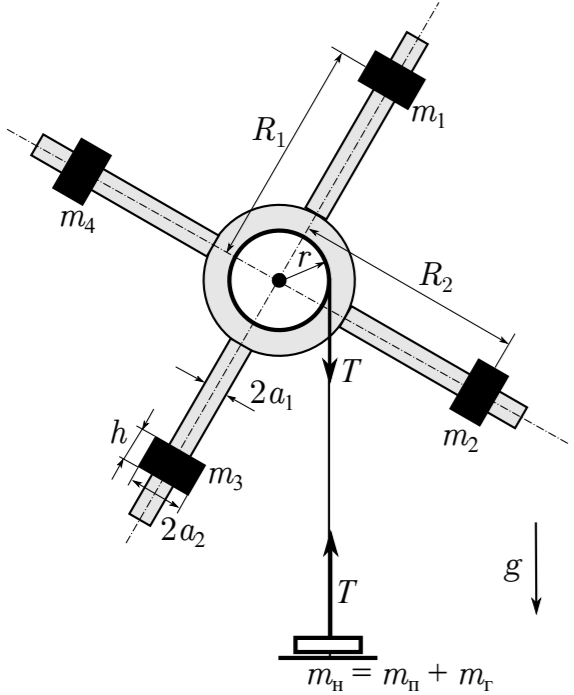
\includegraphics[width=0.5\textwidth]{Маятник}
\end{center}
\caption{Крестообразный маятник Обербека} \label{маятник}
\end{figure}
На маятник действуют два момента сил: силы натяжения нити ($M_T$) и трения ($M_\text{тр}$): $M_T = rT$, $r$ - радиус шкива. Для движения платформы с учетом нерастяжимости нити:
\[m_H \beta r = m_H\ddot{y} = m_Hg - T\]
Откуда согласно основному уравнению вращательного движения:
\begin{equation}
(I+m_Hr^2)\beta = m_Hgr-M_\text{тр}
\label{M_T}
\end{equation}

Рассмотрим момент силы трения. Его зависимость от скорости не ясна, однако может иметь как составляющую, пропорциональную силе реакции в оси $N$ (сухое трение), так и составляющую, пропорциональную угловой скорости вращения (вязкое трение). Откуда:
\begin{equation}
M_\text{тр} \simeq (1 + \frac{m_H}{m_M}) M_0 + \eta \omega \approx M_0 +\eta \omega
\label{трение}
\end{equation} 
где $M_0$ - момент сил трения для покоящегося маятника при нулевой массе подвеса, $m_M$ - масса маятника 

Для расчета момента инерции системы, предположим, что грузы $m_i$ имеют форму полых цилиндров, внутренний и внешний радиус которых известен, образующая h
\begin{equation}
I = I_0 + \sum_{i=1}^4(I_i+m_iR_i^2)
\label{I}
\end{equation}
где $I_0$ - момент инерции системы без грузов, $R_i$ -  расстояние от центров масс грузов до оси вращения
\begin{equation}
I_i = \frac{1}{12}m_ih^2+\frac{1}{4}m_i(a_1^2+a_2^2)
\label{Ii}
\end{equation} - момент инерции груза относительно оси, проходящей через его центр масс
\end{document}